\section{Paket Verlust}
\label{sec:Paket Verlust}

\subsection{Vorgehen bei Paketverlust}

Falls ein Übertragungsmedium nicht korrekt funktioniert, ist es möglich, dass Datenpakete nicht am Ziel oder mit einer zu grossen Verspätung ankommen.
Da jedes \esp{} Paket mit einer Sequenznummer versehen ist, können diese Paketverluste erkannt und gemeldet werden.

Die \esp{} Pakete besitzen zum Schutz vor Replay-Angriffen eine Sequenznummer sowie einen bestimmten Gültigkeitsbereich (Windowsize).\\
Die Pakete können zum Beispiel durch Loadbalancing \"{u}ber unterschiedliche Pfade verschickt werden. Dadurch kann die Reihenfolge der Pakete am Ziel nicht mehr gewährleistet werden. Die zu spät ankommenden Pakete müssen daher überprüft werden, ob die Sequenznummer aktuell noch gültig ist (innerhalb des Window).

\begin{figure}[H]
    \begin{center}
        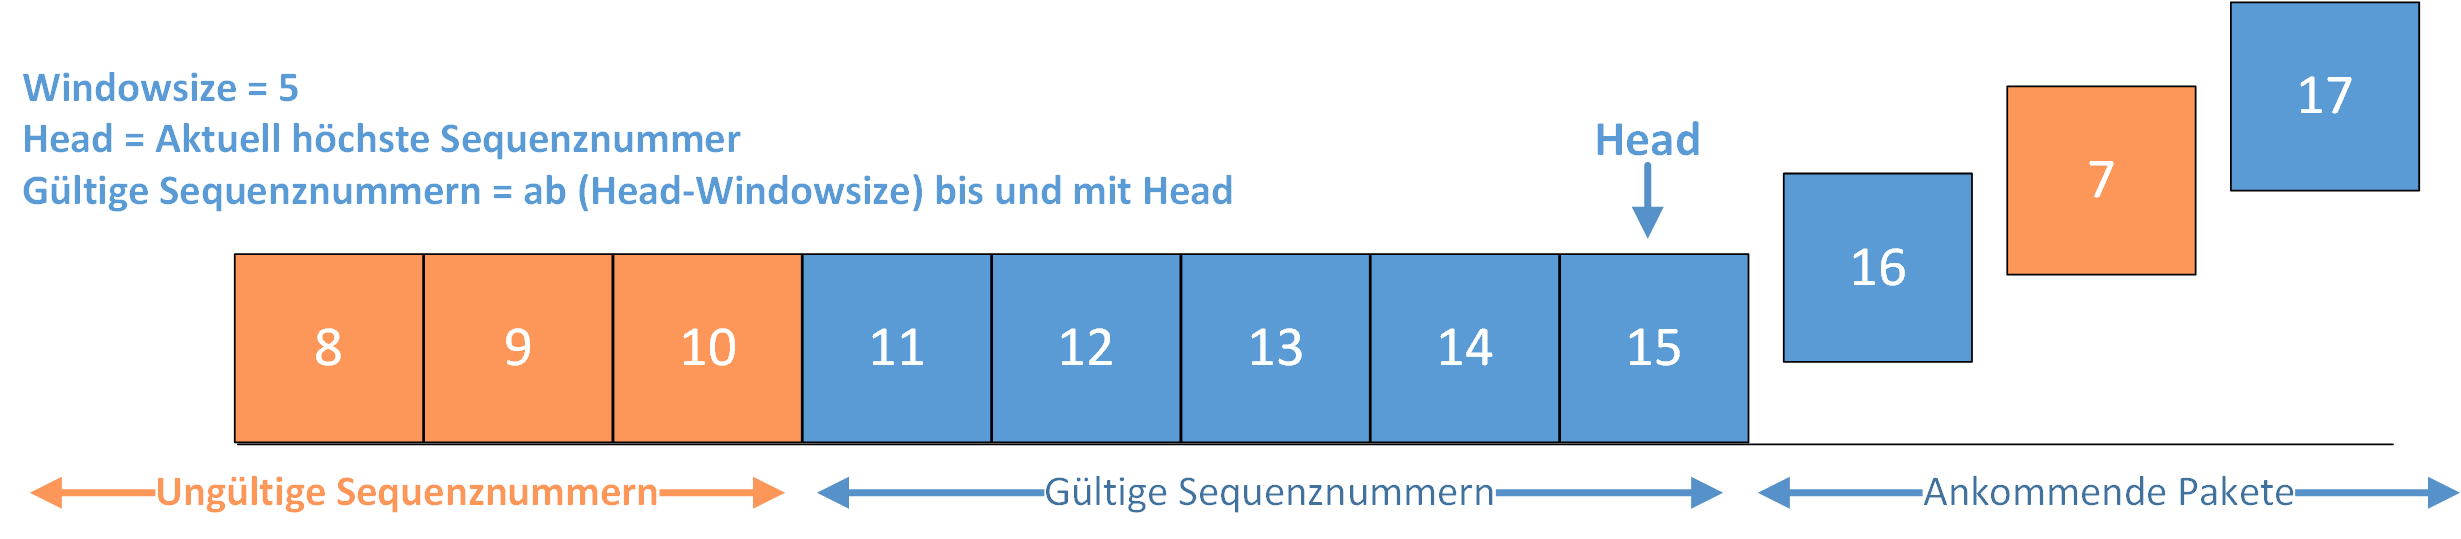
\includegraphics[trim=1 0 0 0,clip,width=\textwidth]{start/img/Sequenznummern.png}
    \end{center}
    \caption{Windowsize und Gültigkeitsbereich}
\end{figure}

Um zu überprüfen ob bei einer VPN-Verbindung Paketverluste auftreten, müssen die Sequenznummern überwacht werden. Hier spielt der Wert von Head(grösste empfangene Sequenznummer) eine wichtige Rolle. Falls eine Sequenznummer eines neuen Pakets nicht um eins grösser ist als der aktuelle Head, wurde eine Verbindung gestört.\\
Nun muss aber ausserdem festgestellt werden ob Pakete verloren oder nur verspätet ankommen. Es braucht daher eine Möglichkeit diese Sequenznummern zu erfassen die bei einer aktiven Verbindung momentan fehlen.\\
Ein weiteres Problem ist die Unterscheidung von Paketen die Ausserhalb des Window, also stark verspätet, oder gar nicht angekommen sind. Diese Information ist wichtig um bei häufigem auftreten von verspäteten Paket mit einer möglichen Erhöhung der Windowsize reagieren zu können. Die Nützlichkeit dieser Information wurde erst nach dem entwickeln eines ersten Prototyps erkannt und darauf implementiert.


Ein Entwurf all dieser Überlegungen sieht wie folgt aus:\\
\begin{figure}[H]
    \begin{center}
        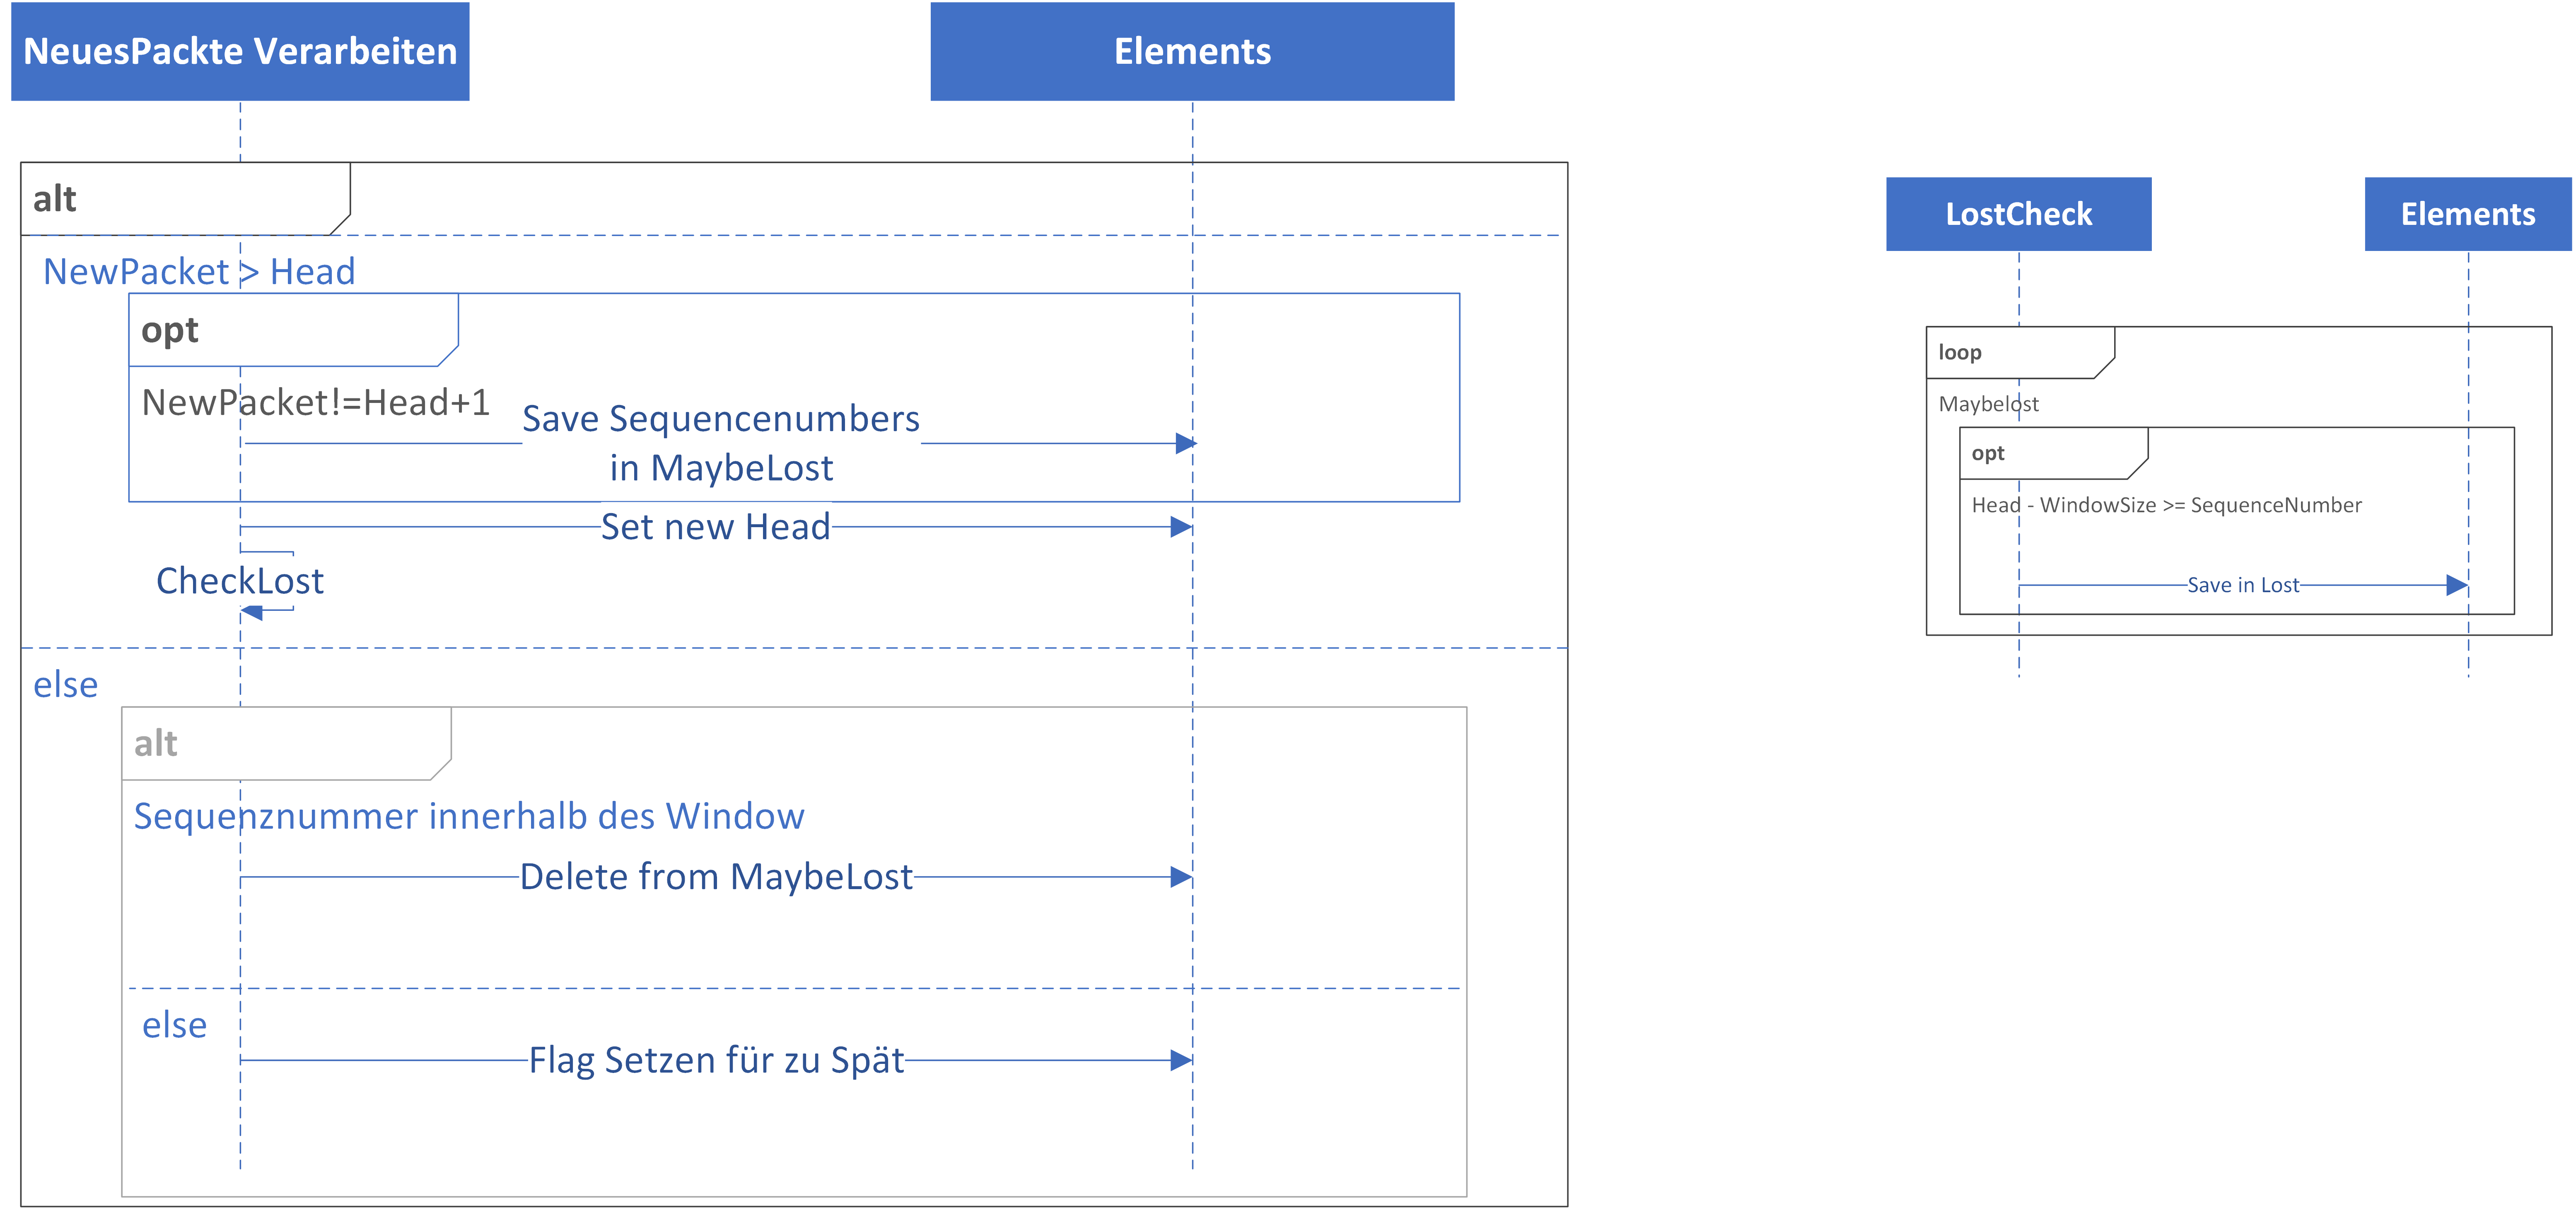
\includegraphics[trim=1 0 0 0,clip,width=\textwidth]{start/img/SequenceDiagramLostPackets_2.png}
    \end{center}
    \caption{Entwurf eines Algorithmus zur erkennung des Paket Verlusts}
\end{figure}

\subsection{Benachrichtigung bei Paketverlust}

Ein zweiter wichtiger Punkt neben dem erkennen eines Paketverlustes ist die Benachrichtigung. Es wurde entschieden eine Syslogmeldung bei Überschreitung eines Grenzwertes zu versenden. Um aber eine solche Meldung möglichst klein zu halten, wurde entschieden gleichzeitig eine Datei mit Detaillierten Informationen zu generieren.\\
Somit kann der Syslog Meldung sofort entnommen werden, um welche Verbindung es sich handelt, welche das Problem verursacht hat. Falls dieses Problem immer wieder bei der gleichen Verbindung auftritt kann die Infodatei eingesehen werden um zu erkennen wie viele Pakete und zu welchem Zeitpunkt Pakete verloren gingen. Zudem werden Informationen geliefert ob Pakete zu spät oder gar nicht angekommen sind.\\
Bei einem ersten Prototyp wurde erkannt, dass es ebenfalls einen Mechanismus benötigt, um ein erneutes versenden des gleichen Alerts zu unterbinden. Da bei jedem ankommenden Paket überprüft wird ob ein Alert versendet werden muss, gab es bei Verbindungen mit einem hohen Paketverlust eine Flut von Alert Nachrichten. Um dieses Problem zu unterbinden, wurde eine Barriere eingebaut diese lässt ein verschicken derselben Nachricht nur alle 10 Sekunden zu. Hinzu kommt ein Mechanismus Syslogservern, welcher Nachrichten blockt die gerade geloggt wurden.\\

\subsection{Konfigurierte Werte}
Folgende Werte sind in Zusammenhang mit dem Paketverlust konfigurierbar:

\begin{itemize}
  \item \textbf{SyslogServer:} Die Adresse des Syslogservers inklusive Port. An diesen Server werden die Alertnachrichten gesendet.
  \item \textbf{WindowSize:} Die grösse des ESP-Window. Standardmässig ist eine grösse von 32. 
  \item \textbf{AlertTime:} Die Zeitdauer innerhalb die Paketverluste gezählt werden. Beispiel 10: Es wird überprüft ob in den letzten 10 Sekunden AlertCounter überschritten wurde. Bei Überschreitung wird ein Alert versendet.
    \item \textbf{AlertCounter:} Die Anzahl Pakete ab welcher ein Alert versendet wird.
  \item \textbf{PcapFile:} Falls dieser Wert gesetzt wurde, wird nicht der Paketverlust einer Live Verbindung ermittelt, sonder der Paketverlust eines PcapFiles. Dadurch sind Tests mit dem Tool wiederholbar und können nachvollzogen werden.
\end{itemize}